
\chapter{Analyse der spannkraftinduzierten Deformation}

Im folgenden Kapitel wird die Methode zur Erkennung und Analyse von durch 
Spannkraft induzierter Deformationen beschrieben. Ziel ist es, 
aus zwei zusammengefügten Bilder von zwei verschiedenen Spannungsstufen, 
eine Deformation zu erkennen und auszugeben.
Als Deformation wird eine äußerliche Veränderung des betrachteten Bauteils bezeichnet, 
die äußere Veränderung ist hierbei über den Unterschied der Ränder der Bauteile definiert.
Bevor also eine Deformation erkannt werden kann, muss die Randgeometrie von beiden
abgebildeten Bauteils erfasst werden.
Vorerst werden in einem Schritt immer nur zwei Spannungsstufen miteinander verglichen 
und die Deformationsdaten anschließend abgespeichert.
Die Auswertung der resultieren Daten erfolgt in einem separaten Schritt, so können auch
mehrere Spannungsstufen untereinander verglichen werden, ohne die Deformationserkennung 
komplexer zu machen.

\section{Deformation zwischen zwei Spannungszuständen}

Wie schon erwähnt ist die Deformation zwischen zwei Bauteilen als Differenz der 
Randgeometrie deformiert. Um die Randgeometrie eines Bauteils zu ermitteln, 
kann wieder die Kontursuche angewendet werden. Die gefundenen Konturen bilden dann 
das Bauteil ab. So werden äußere aber auch innere Geometrie abgebildet und machen die 
Deformationserkennung möglich. In Abbildung \ref{fig:stichted_contour} ist ein 
zusammengefügtes Bild und die erkannte Randgeometrie eines Bauteils zu sehen.

\begin{figure}[H]
    \centering
    \begin{minipage}{0.49\textwidth}
        \centering
        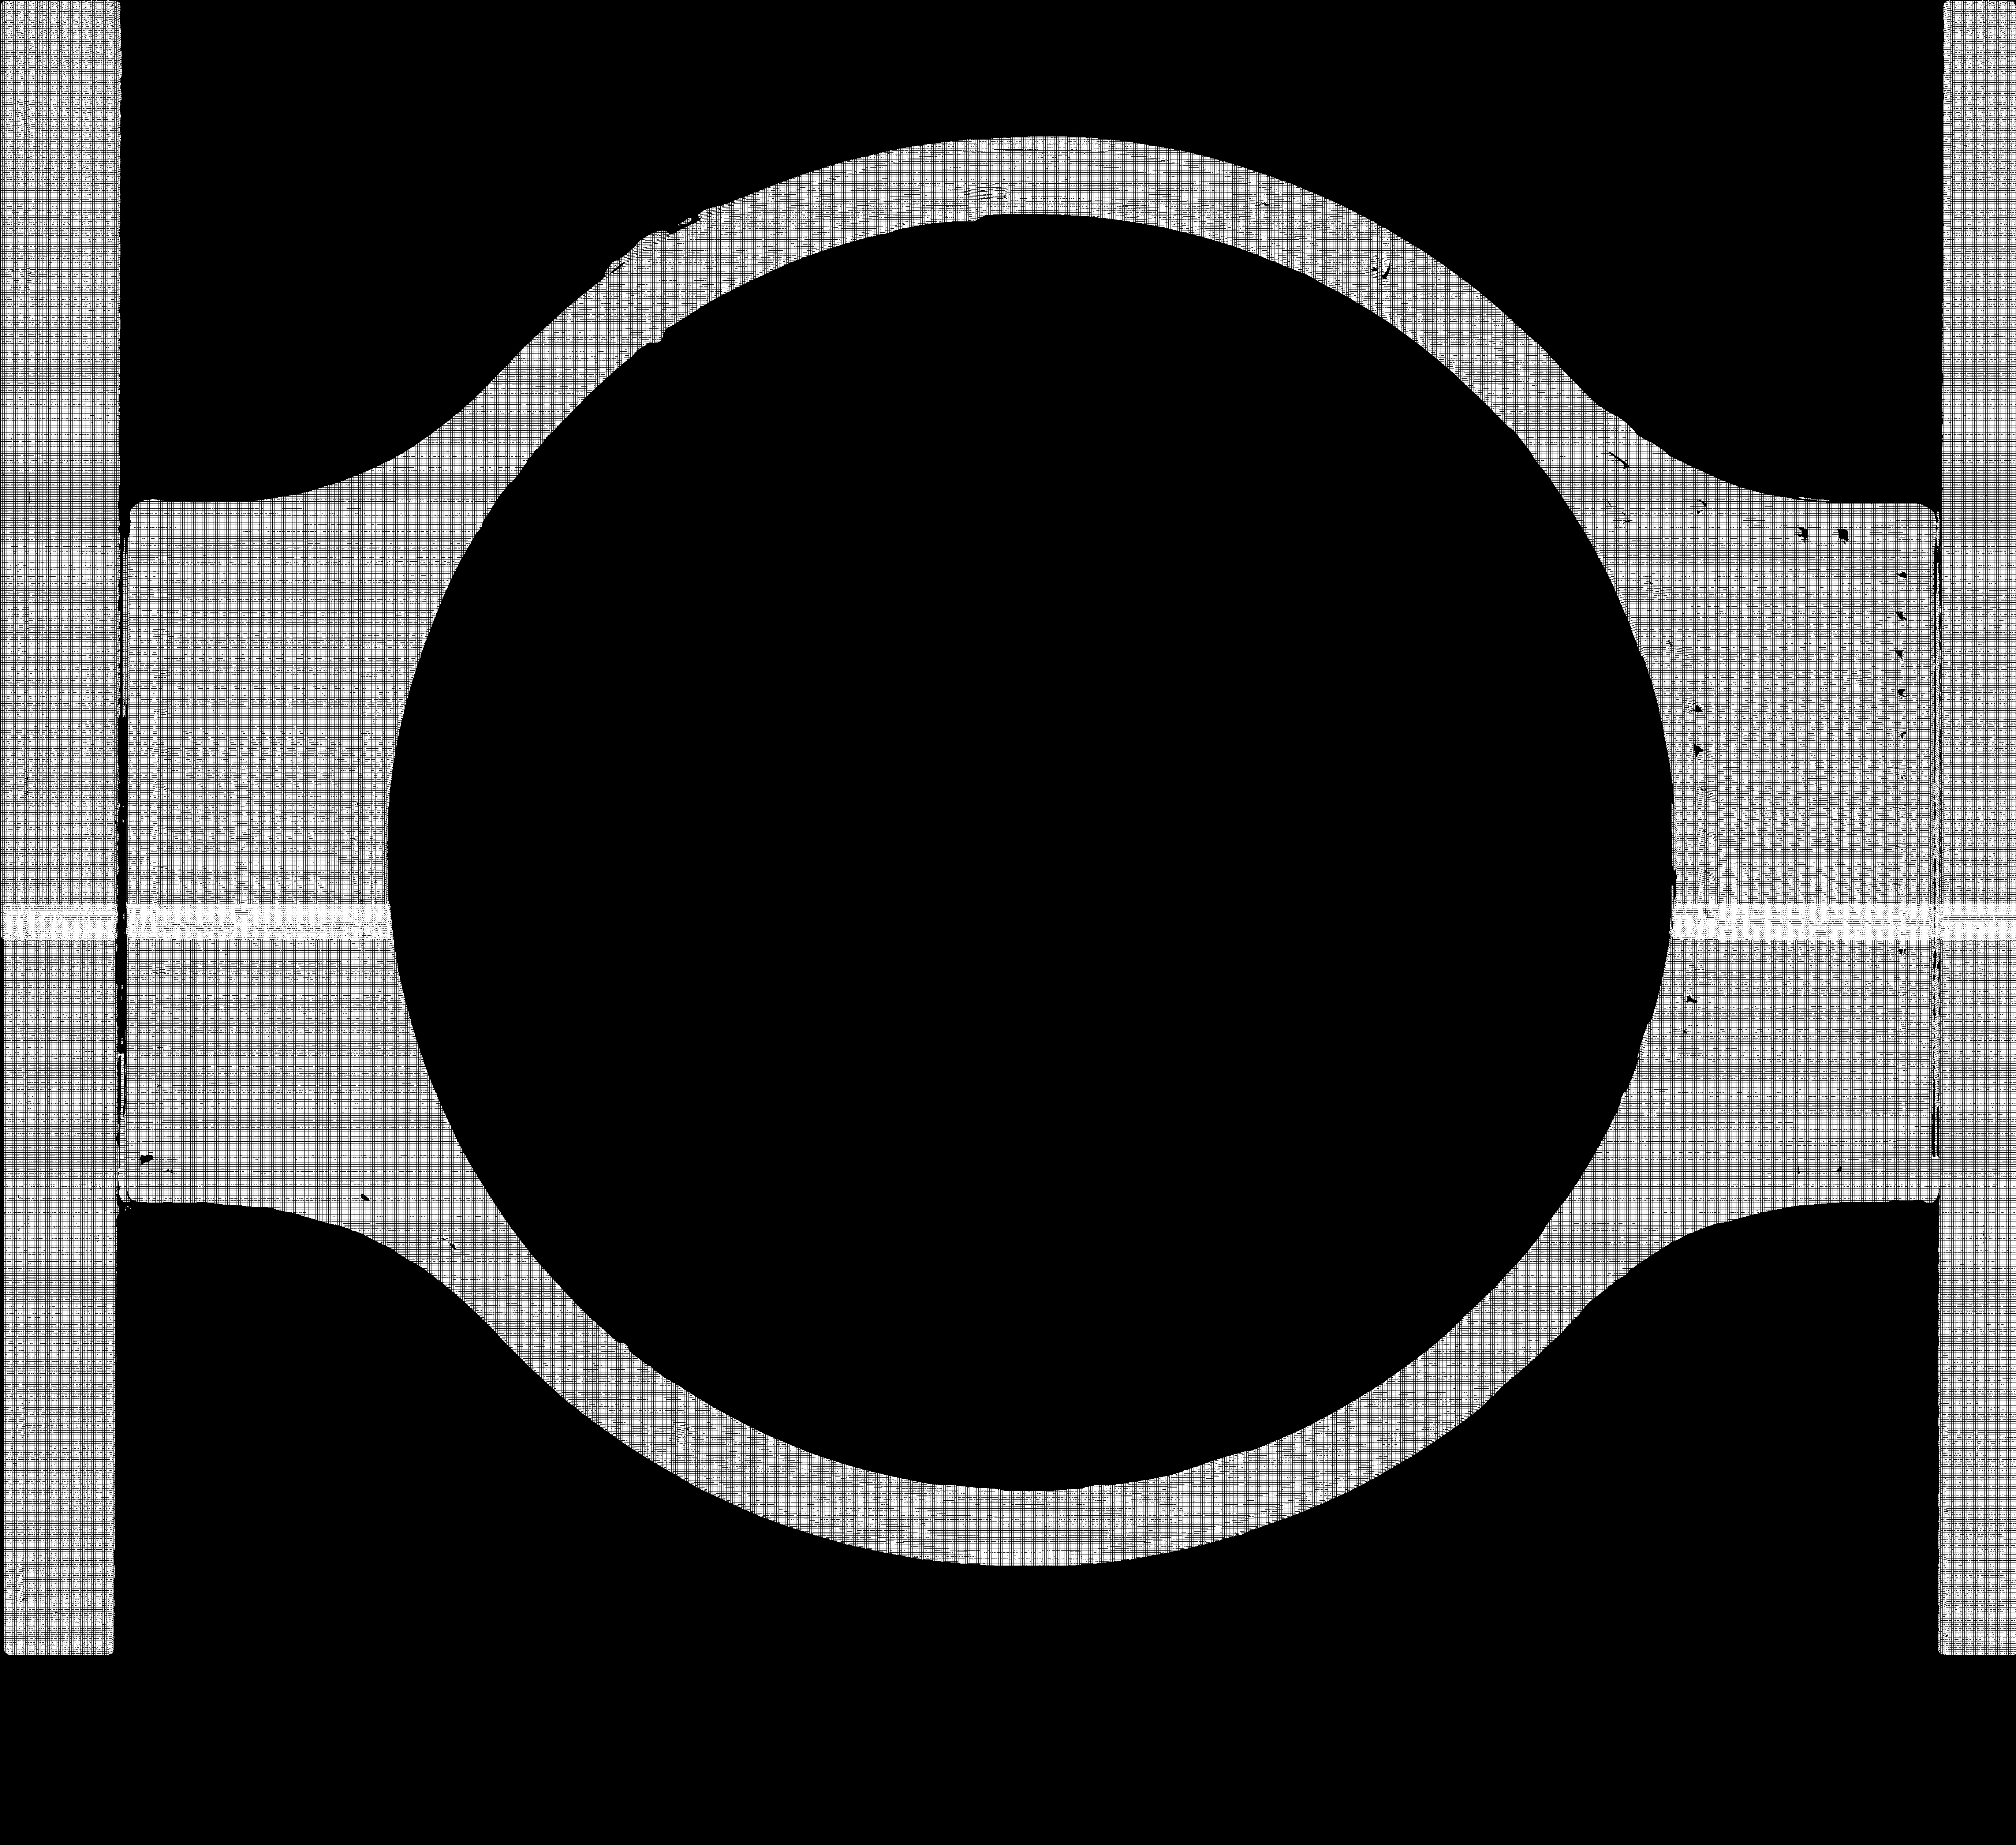
\includegraphics[width=\textwidth]{images/FDM_sp0_stitched.jpg} % first figure itself
        \caption*{(a)} 
    \end{minipage}\hfill
    \begin{minipage}{0.49\textwidth}
        \centering
        \includegraphics[width=\textwidth]{images/contours_FDM_sp0_stitched.jpg} % first figure itself
        \caption*{(b)}
    \end{minipage}\hfill
    \caption{(a) Zusammengefügtes Bild des FDM Demonstratorbauteils, Spannungsstufe 0
    (b) Randgeometrie von (a), die zur Erkennung der Deformation genutzt wird}
        \label{fig:stichted_contour}
\end{figure}

Um die Differenz zweier Randgeometrien bilden zu können, müssen diese angenähert werden.
Dies garantiert, dass die gebildete Differenz minimal ist.
Der schon beschriebe Ansatz des Kontourmatching könnte auch hier genutzt werden. 
Allerdings müssen hier die gesamten Konturen betrachtet werden und nicht wie zuvor nur 
der überlappende Auschnitt. Das schon vorgestellte Verfahren ist für die Konturen eines
gesamten Bauteils nicht performant genug um eine akzeptable Wartezeit für das Verfahren
zu gewährleisten. 
Deswegen wird hier ein anderes Verfahren eingesetzt. Es basiert auf demselben Prinzip,
Punktepaare zu finden deren euklidischen Distanz gleich null ist. Anstatt das aber 
jeder Punkt der Zielkontur mit jedem Punkt der Ursprungskontur verglichen wird, 
wird ein maximaler Radius definiert in dem nach benachbarten Punkten gesucht wird.
Hierfür muss die Kontur erst in eine zweidimensionale Datenstruktur überführt werden.
Dieser zusätzliche Aufwand lohnt sich wegen einer deutlich verkürzten Laufzeit.

Ähnlich zu dem schon beschriebenen ICP-Algorithmus wird eine Transformation berechnet,
mit der die eine Kontur der anderen Kontur angenähert werden kann.
Die Transformation wird mit folgendem Algorithmus gebildet:
(FRAGE: Hier entweder das, oder latex-pseudocodeblock, oder python screenshot?)
\begin{enumerate}
    \item Zu jeden Punkt in der Ursprungskontur wird der Nachbarpunkt,
    der Zielkontur gesucht der den kleinsten euklidischen Abstand besitzt.
    \item Wird kein Punkt in einem definierten Radius gefunden wird der nächste Punkt
    betrachtet. Falls ein Punkt gefunden wurde, wird der Vektor gebildet der beide Punkte
    verbindet.
    \item Wenn alle Punkte der Kontur betrachtet sind, wird der Durchschnitt aller gefunden
    Vektoren gebildet.
    \item Da die Transformation auf Pixel angewendet wird, muss sie ganzen Zahlen 
    entsprechen. Wenn der Absolutwert beide Vektorelemente der Transformation 
    unter 0.2 Pixel fallen wird die Transformation auf (0, 0) gerundet. 
    Ansonsten wird auf die nächstgrößere (oder kleinere bei negativen Werten) ganze 
    Zahl gerundet.
\end{enumerate}

Ist die Transformation ungleich dem Vektor (0,0) wird sie auf die Ursprungskontur 
angewendet und erneut die Transformation berechnet. Dies wird so lange wiederholt bis 
die Transformation dem Nullvektor entspricht. Wenn dies geschieht, sind beide Konturen, 
und damit die Randgeometrien der Bauteile angenähert.
Um Rechenzeit zu sparen werden vor dem Ermitteln der ersten Transformation die 
Massenmittelpunkte beider Bauteilgeometrie berechnet und Übereinader gelegt.

Nachdem die beschriebenen Schritte erfolgt sind, kann die Deformation bestimmt werden.
